%\documentclass[conference]{IEEEtran}
\documentclass{article}
\usepackage[hidelinks]{hyperref}
\usepackage{todonotes}
\usepackage{graphicx}
\usepackage{tabularx}
\usepackage{amsmath}
\usepackage{cite}

\newcommand{\ecomment}[1]{\todo[inline, color=red!40]{Ettore: #1}}

\begin{document}

\title{AILEC3 - Artificial Intelligence for Lower Energy Consumption in Cloud Computing}

\author{
%\IEEEauthorblockN{Ettore Tancredi Galante}
%\IEEEauthorblockA{\textit{Department of Computer Science} \\
\textit{Ettore Tancredi Galante} \\
\textit{Department of Computer Science} \\
\textit{University of Milan} \\
\textit{Milan, Italy} \\
ettoretancredi.galante@studenti.unimi.it
}


%\IEEEoverridecommandlockouts
%\IEEEpubid{\makebox[\columnwidth]{978-1-6654-3886-5/21/\$31.00~\copyright2021 IEEE \hfill} \hspace{\columnsep}\makebox[\columnwidth]{ }}
\maketitle
\newpage
\tableofcontents
\newpage
%\IEEEpubidadjcol

\pagenumbering{arabic}
\section{Abstract}\label{sect:abstr}

\ecomment{Placeholder for the abstract.}
\section{Introduction}\label{sect:intro}

The widespread adoption of \textit{cloud computing} services in the last few years has led to a significant increase in the energy consumption 
of \textit{data centers}, which has become a critical concern for cloud providers. 
While cloud computing offers many benefits, such as cost savings and scalability, 
the energy consumption associated with it has negative implications both from an environmental and financial perspective. 
As the demand for cloud services continues to grow, the energy consumption of data centers is expected to increase exponentially, 
further exacerbating the issue.

The optimization of resource allocation in \textit{cloud computing environments} is a complex problem that involves a large number of variables and constraints. 
The main objective is to minimize energy consumption while maintaining or improving the performance of the services. 
Achieving this goal is challenging due to the scale of cloud computing infrastructures, the dynamic nature of workloads, and the need to provide 24/7 availability. 
Given these challenges, cloud providers face the dilemma of how to maintain high-quality service delivery while reducing energy consumption.

\textit{Artificial Intelligence} (AI) techniques, such as \textit{genetic algorithms}, have been widely studied as a method for addressing this problem. 
% ^^^ Insert citations here

Genetic algorithms are a type of optimization algorithm that mimic the process of natural evolution and use heuristic techniques to find near-optimal solutions 
for complex problems. Genetic algorithms are well suited for solving problems that involve a large number of variables and constraints, 
such as the resource allocation problem in cloud computing. They can explore a large search space in a relatively short amount of time, 
enabling them to find near-optimal solutions even when faced with incomplete or uncertain information.

The use of genetic algorithms in cloud computing has the potential to significantly improve the energy efficiency of data centers while maintaining or improving performance. 
By optimizing resource allocation, genetic algorithms can reduce the number of servers and storage devices required to run a given workload, 
which in turn reduces energy consumption. Additionally, genetic algorithms can adapt to changes in workload and resource usage patterns, 
further improving the energy efficiency of the data center.

One of the key challenges of measuring energy consumption in cloud computing is identifying the power consumption of the various components of the system, 
such as servers, storage devices, and network devices. 
The energy consumption of these components is typically measured in watt-hours (Wh) or joules (J). 
The energy consumption of a data center can be measured at different levels of granularity, from individual servers to entire racks or data centers. 
One of the most commonly used metrics for measuring energy consumption in cloud computing is \textit{Power Usage Effectiveness} (PUE). 
PUE is a ratio of the total energy consumed by a data center to the energy consumed by the IT equipment. 
A PUE of 1.0 indicates that all of the energy consumed by the data center is used by the IT equipment, while a PUE of greater than 1.0 
indicates that some of the energy is being used for other purposes, such as cooling and lighting.

Despite the advantages of using genetic algorithms for resource allocation in cloud computing, there are also limitations to consider. 
One of the main limitations is the computational expense of genetic algorithms, particularly when the problem size is large. 
The resource allocation problem in cloud computing environments can involve a large number of variables and constraints, 
which can make the computational cost of genetic algorithms quite high. This can make them impractical for certain types of problems or when resources are limited. 
Additionally, genetic algorithms are often sensitive to the choice of parameters and initial conditions. This can make it difficult to obtain consistent and reliable results, 
as the choice of parameters and initial conditions can have a significant impact on the performance of the algorithm.

The selection of suitable parameters and initial conditions is an important step in the implementation of genetic algorithms. 
It requires a significant amount of expertise and experience to choose the appropriate parameters and initial conditions that will lead to good performance. 
Furthermore, the results obtained from genetic algorithms are probabilistic in nature, which means that multiple runs of the algorithm are typically required 
to obtain a stable and robust solution. This can increase the computational cost and time required to obtain a solution, which can be a limitation when resources are limited.

In addition to computational expense and sensitivity to parameters, genetic algorithms also have some other limitations such as the lack of guarantee of global optima, 
and the risk of getting stuck in local optima. Genetic algorithms are also not suitable for problems with deterministic solutions. 
Furthermore, the stochastic nature of genetic algorithms may also lead to a lack of reproducibility of results. 
These limitations must be taken into account when deciding to implement genetic algorithms in cloud computing environments.

However, the potential benefits of using genetic algorithms in cloud computing outweigh the limitations. 
Genetic algorithms have the potential to significantly improve the energy efficiency of data centers while maintaining or improving performance. 
By optimizing resource allocation, genetic algorithms can reduce the number of servers and storage devices required to run a given workload, 
which in turn reduces energy consumption. Additionally, genetic algorithms can adapt to changes in workload and resource usage patterns, 
further improving the energy efficiency of the data center.

To effectively use genetic algorithms in cloud computing, cloud providers need to carefully evaluate the trade-offs between the potential benefits and limitations of using these algorithms. 
Cloud providers must consider the specific characteristics of the problem at hand, the computational resources and expertise available, 
and the potential benefits of using genetic algorithms in their environment. 
The use of genetic algorithms requires a significant amount of expertise and experience to choose the appropriate parameters and initial conditions 
that will lead to good performance. Cloud providers must have a thorough understanding of the characteristics of the problem they are trying to solve, 
and they must be prepared to invest significant time and resources in the development and implementation of genetic algorithms.
%\section{State of the Art}\label{sect:sota}
\section{Dataset}\label{sect:dtst}
%\section{Outlining the problem}\label{sect:problem}

The problem here described is a problem of optimization. 
The goal is to find an acceptable solution by using a genetic algorithm to the assignation of a set of processes to a set of servers.
The problem is defined as follows:\\
A Servers $s$ has a CPU speed $cs$, calculated in Gigahertz (GHz) and a number of CPUs $cn$.\\
A Process $p$ has a length $l$, calculated in number of instructions.\\
A Solution $sol$ is a collection of tuples $(s_n, [p_1, p_2, ..., p_m])_{n}$ where $s_n$ is the $n^{th}$ Server of the tuple 
and $[p_1, p_2, ..., p_m]$, with variable $m$ for each tuple, is a list of Processes.\\
Let's define, for a Server, the following functions:
\begin{itemize}
    \item $cs(s)$: CPU speed of the Server $s$;
    \item $cn(s)$: Number of CPUs of the Server $s$.\\
\end{itemize}
For a process, we define the following function:
\begin{itemize}
    \item $l(p)$: Length of the Process $p$.\\
\end{itemize}

For a solution $sol$, The fitness function $f$ of $sol$ is defined as follows:
\begin{equation}
    \label{fitness}
    f(sol) = \sqrt{\sum_{0}^{n}{(\sum_{0}^{m}l(p_m) * (cs(s_n) * cn(s_n)))^2}}
\end{equation}
%$$f(sol) = \sqrt{\sum_{0}^{n}{(\sum_{0}^{m}l(p_m) * (cs(s_n) * cn(s_n)))^2}}$$

\section{Baseline}\label{sect:baseline} 

The baseline algorithm defined in this study is a standard genetic algorithm (GA)~\cite{mitchell1998introduction} that is used to optimize 
process allocation in cloud computing environments. The idea is that by optimizing the process allocation, the energy consumed by the cloud envirnoment is minimized as well.
The GA is a stochastic population-based search algorithm that is based on the principles of natural selection and genetics.
It is a meta-heuristic that is used to find approximate solutions to optimization problems.~\cite{kramer2017genetic}

The GA is composed of the following components:
\begin{itemize}
    \item A population of candidate solutions;
    \item A fitness function that is used to evaluate the quality of each candidate solution;
    \item A selection operator that is used to select candidate solutions for reproduction;
    \item A crossover operator that is used to combine the selected candidate solutions to produce new candidate solutions;
    \item A mutation operator that is used to introduce random changes to the candidate solutions;
    \item A termination criterion that is used to determine when the GA should stop searching for solutions.
\end{itemize}

\begin{figure}[h]
    \centering
    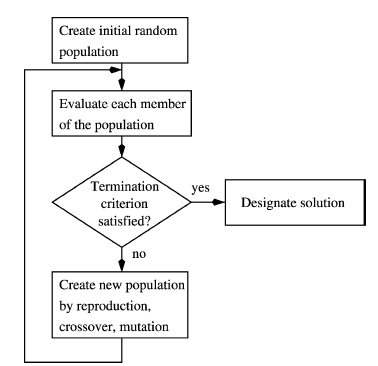
\includegraphics[width=0.5\textwidth]{./resources/examples/GAWorkflow.png}
    \caption{How a Genetic Algorithm works.}
    \label{fig:baseline}
\end{figure}
How a Genetic Algorithm (GA) works is shown in the flowchart~\cite{gaworkflow} shown in Figure~\ref{fig:baseline}.

In this setting, the candidate solutions are represented by a list of tuples, each of which contains a Server and a list of Processes.
The initial population is generated by iterating over the Server list. 
For each Server, from the list of all the Processes, iteratively, a process is selected at random with probability $$p = \frac{1}{n}$$
with $n$ being the number of servers taken into account in the solution. As a Process is selected, it is removed from the global Process list.

Then, the fitness function~\eqref{fitness}, is used to evaluate the quality of each candidate solution.

% Discuss about the parameters of the GA
The baseline genetic algorithm has been tested over a pletora of parameters, in order to find the best combination that would lead to acceptable results.
The parameters that have been tested are:
\begin{itemize}
    \item The probability of selecting a process for a server;
    \item The crossover rate;
    \item The probability of mutation;
    \item The population size;
    \item The number of generations.
\end{itemize}

The selection probability $p_s$ is equal to $\frac{1}{\#_{servers}}$. In the first settings of the experiments this value was 
set in different ranges between $[0.3, 0.6]$, but this not only led to a very slow convergence of the GA but produced undesired noise
in the results in most of the experiments.
The crossover rate $p_c$ is set to $0.9$. A starting value of $0.5$ was used, but this led to unsatisfactory results, opposed to what~\cite{mirjalili2019genetic} claimed
in their research.
Better results were obtained by increasing the crossover rate to $0.7$, but the best ones were yield by $p_c = 0.9$, supported by~\cite{hassanat2019choosing}.
The probability of mutation $p_m$ has been initially tested in the range $[0.1, 0.3]$. However, as found in previous research works,
a mutation rate over $0.01$ is a synonym of heavy noisy training epochs and close to no convergence. In fact, it has been found that 
the optimal values for the mutation rate ranges in $[0.005, 0.05]$ for a population size $s_p$ between $100$ and $200$ individuals.~\cite{patil2015optimal}
It follows that the chosen parameters for the mutation rate are $p_m = 0.01$ and $s_p = 200$.

As for the number of epochs employed, for both hardware constraints and time reasons, the GA has been run for a maximum of $500$ generations.
For each experiment, the GA is run $10$ times and the results are averaged in order to obtain an insightful overlook of the performances.

The baseline algorithm has been created to be initially compared to a greedy assignation method of simple ideation.
The fitness function employed in the baseline algorithm has been used to compare the results between the greedy method and the baseline algorithm.


\begin{figure}[ht]
    \centering
    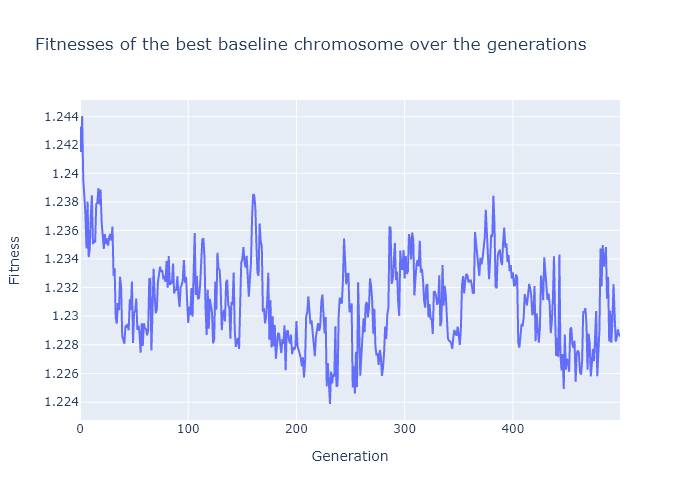
\includegraphics[width=0.75\textwidth]{../../../Code/Genetic/results/baseline/graphs/pop_size_200/500_epochs/average_fitness.png}
    \caption{The average of the Baseline Algorithm over $500$ epochs}
    \label{fig:average_baseline}
\end{figure}


As it can be seen from the results in Figure~\ref{fig:average_baseline}, the fitness function evaluated with the baseline algorithm shows promising results
in a time range comprised between $200$ and $250$ epochs, with its minimum at $231$.
The worst average value of the fitness function in the baseline algorithm is reached in the $2nd$ training epoch, and it is equal to $1.244$.
Moreover, the best average value is reached in the $231th$ epoch, and it is equal to $1.224$.

% Create a table with 10 rows and 2 columns. 
% On the left columns there is written Server X with X ranging from 0 to 9.
% On the right columns there is written the average fitness value for the server X. 
% There is an eleventh row with two columns that has on the left "Magnitude" and on the right the magnitude.
% The table should be centered and the caption should be below the table.

\begin{table}[ht]
    \centering
    \begin{tabular}{|c|c|}
        \hline
        Server & Average Fitness \\
        \hline
        Server 0 & 0.447 \\
        Server 1 & 0.415 \\
        Server 2 & 0.444 \\
        Server 3 & 0.204 \\
        Server 4 & 0.420 \\
        Server 5 & 0.331 \\
        Server 6 & 0.394 \\
        Server 7 & 0.425 \\
        Server 8 & 0.208 \\
        Server 9 & 0.495 \\
        \hline
        Magnitude & 1.233 \\
        \hline
    \end{tabular}
    \caption{The average fitness for each server and the magnitude of the fitness vector.}
    \label{tab:average_greedy_fitness}
\end{table}

When the values are compared to the ones of the greedy algorithm in Table~\ref{tab:average_greedy_fitness}, it can be seen that the baseline algorithm
performs slightly better, since the two magnitudes of the fitness vectors are quite close to each other.
However, the simple baseline genetic algorithm outperforms the greedy technique.\\

Since this experimentation has been carried out with different measures of the fitness function, it is difficult to compare the results to the ones achieved
by other researchers. However, it is possible to compare the results of the different paradigms, algorithms and metaheuristics in order to get a broader picture of the
possible best approaches to adopt in order to solve the problem.
In literature, many works do pair the effectiveness of genetic algorithms paired to greedy techniques. More often than not the latter, despite performing in a less
than optimal way in these scenarios, can be used to improve the capabilities of GAs to obtain even better performances.~\cite{AHUJA2000917}

\newpage
\section{Experiments}\label{sect:exps}


\section{Results}\label{sect:results}

\ecomment{Parlare dei risultati ottenuti, confrontare le tabelle, descrivere l'approccio più promettente.}
\section{Conclusions}\label{sect:conclusions}
\section{Appendix}\label{sect:apdx}
%\input{networks.tex}
%\input{experiment.tex}
%\section{Conclusions}\label{sect:conclusions}

\bibliographystyle{abbrv}
\bibliography{local}

\end{document}